\documentclass[12pt]{article}

\usepackage{linlib}
\usepackage{geometry}
\usepackage{graphicx}

\usepackage{linlib}
\setsansfont[
    Scale=MatchLowercase,
    SmallCapsFeatures={Numbers=Proportional},
    Extension=.otf,
    Path=../fonts/,
    UprightFont=*-Regular,
    BoldFont=*-Bold,
    BoldItalicFont=*-BoldIt,
    ItalicFont=*-It,
]{SourceSans3}

\geometry{
%paperwidth=16.694in,
%paperheight=11.417in,
margin=0.75in,
paperwidth=15.18in,
paperheight=10.25in,
%margin=0.625in,
}

\begin{document}
\sffamily
\pagestyle{empty}

\newdimen\spinewidth
%\spinewidth=1.119in
\spinewidth=0.93in

\newdimen\gutterwidth
\gutterwidth=0.5in

\newdimen\coverwidth
\coverwidth=\dimexpr (\textwidth - \spinewidth) / 2 - \gutterwidth \relax

\setbox0=\hbox{%
    \hskip -0.75in
%\hskip 2.45in
    \lower 2.7in\hbox{%
        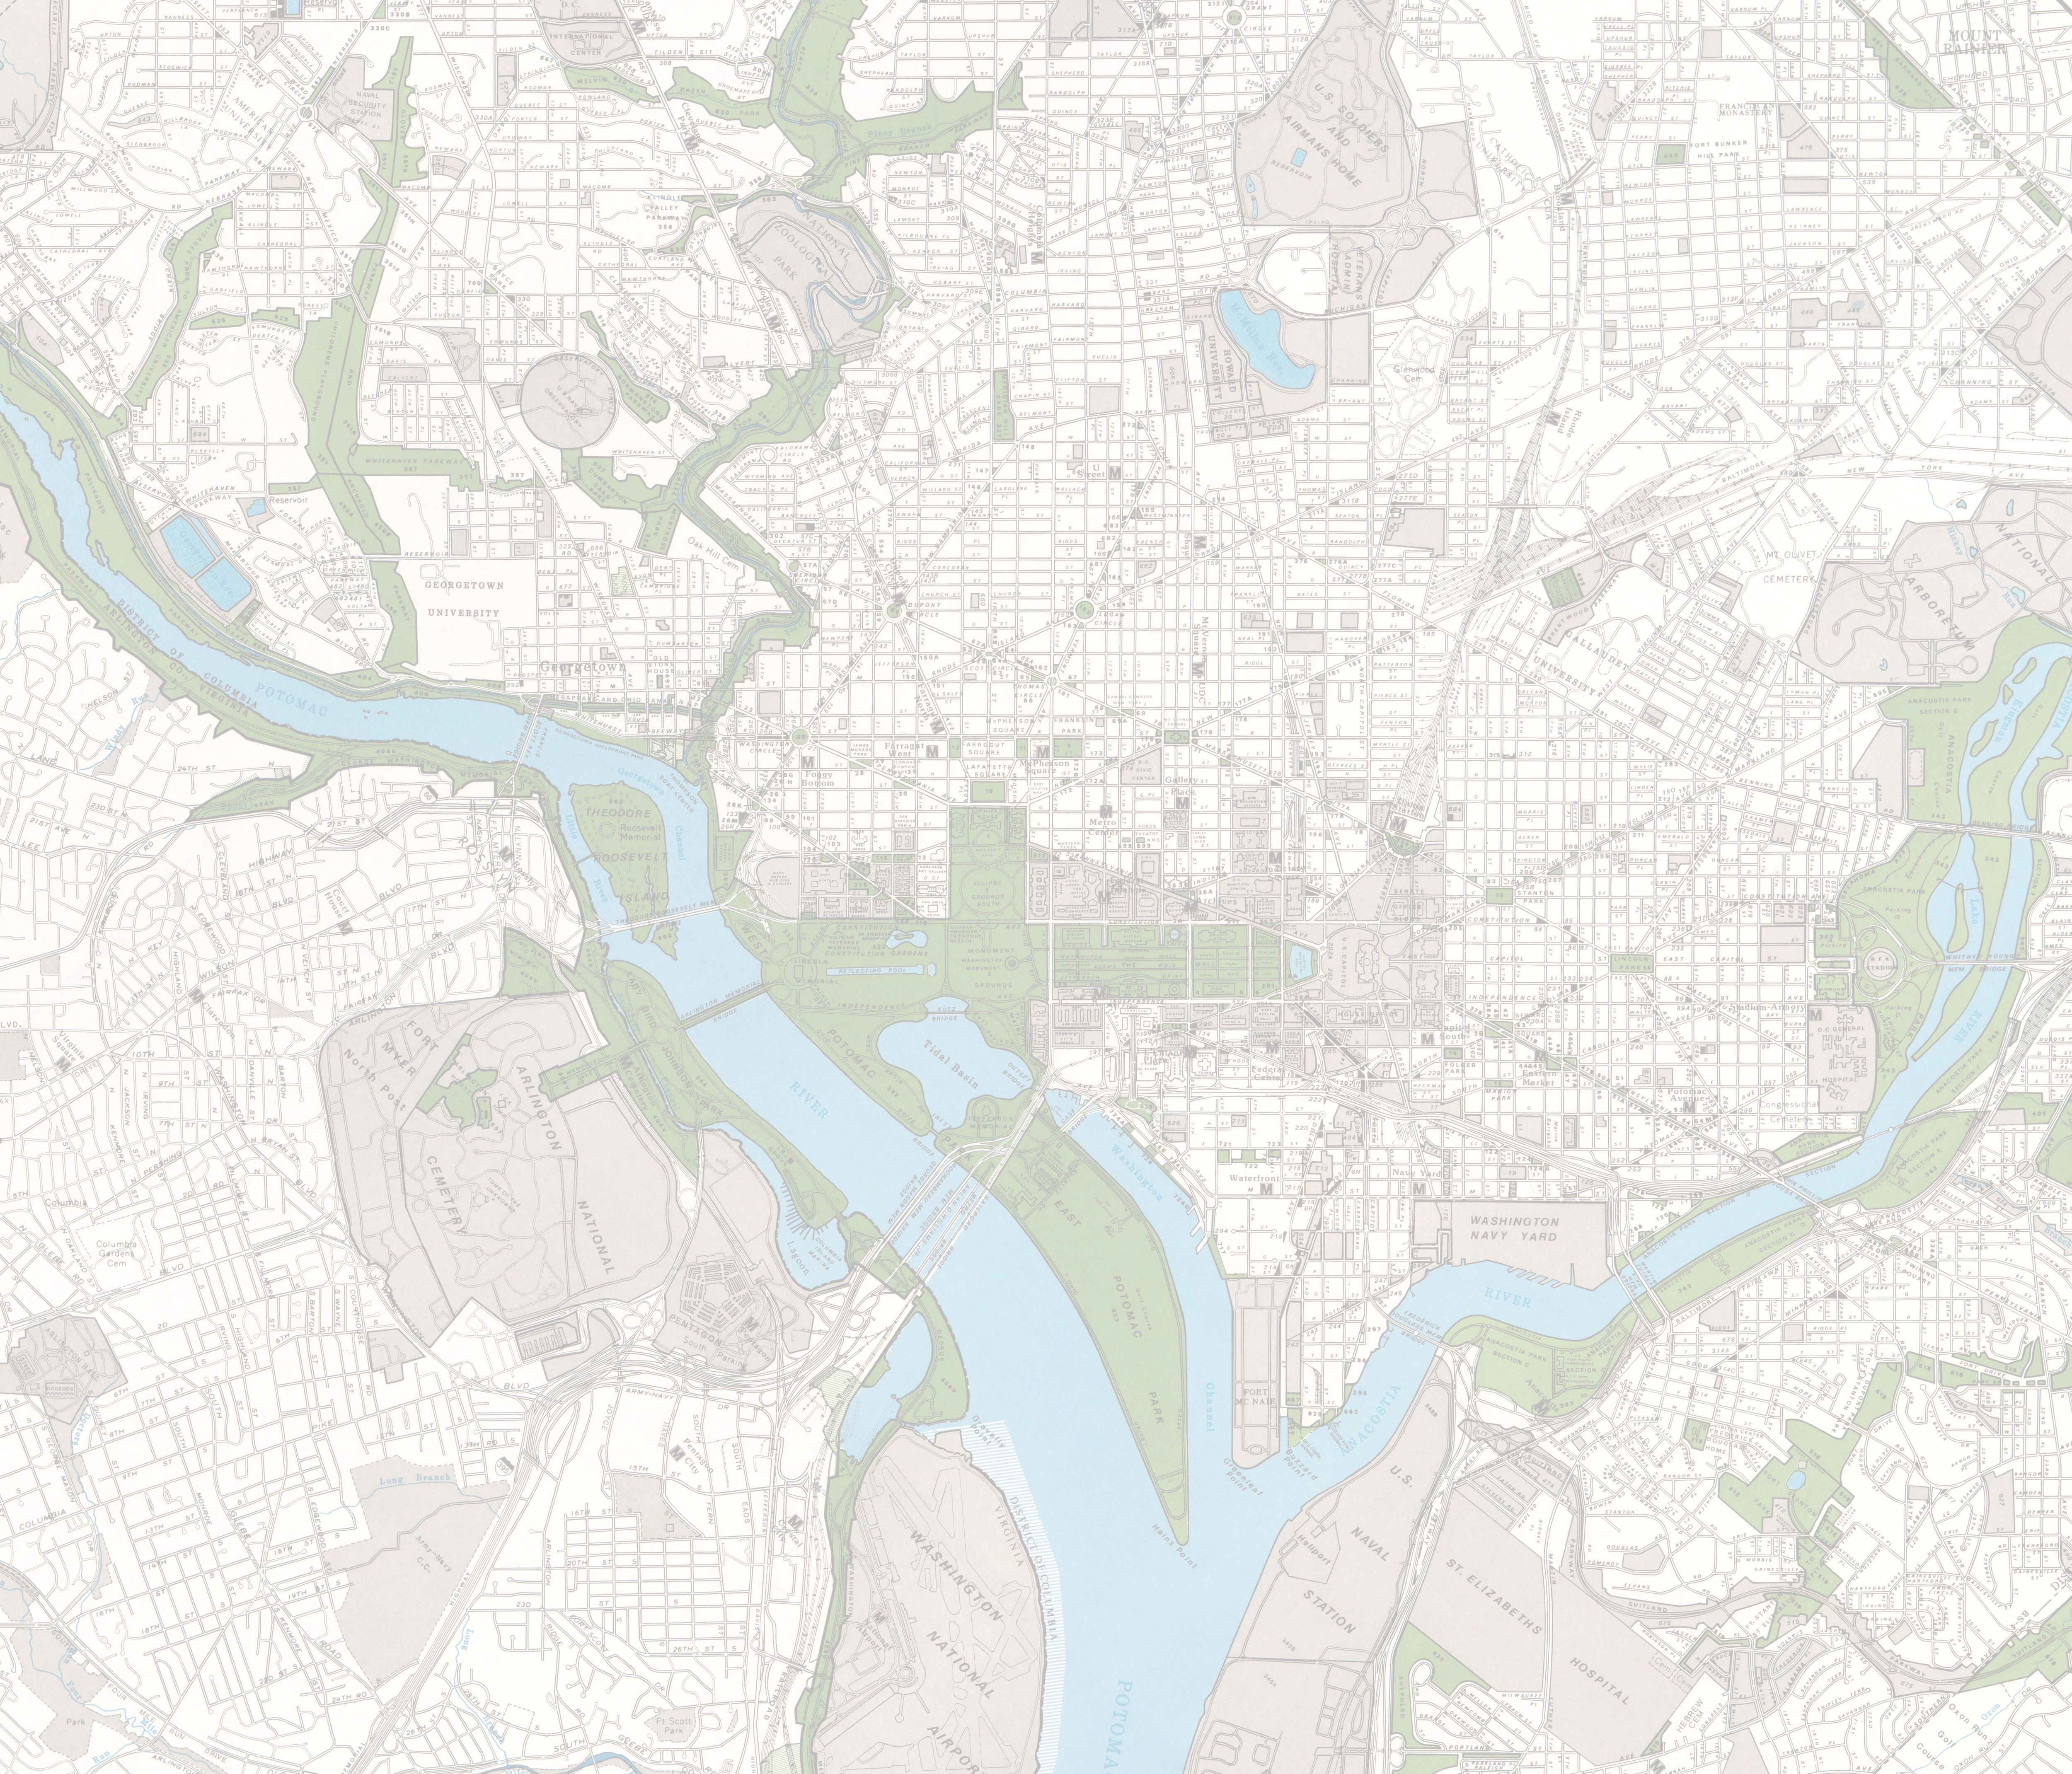
\includegraphics[width=\paperwidth]{national-parks-small.jpg}%
    }%
}
\wd0=0pt
\ht0=0pt
\dp0=0pt

\hbox to \textwidth{%
    \box0
    \vbox to \textheight{%
        \hsize=\coverwidth
        \hbox to \hsize{\hfill}
        \vfill
    }\hfil
    \hbox to \spinewidth{%
        \hfill
        \rotatebox[origin=br]{-90}{\hbox to \textheight{%
            \Huge\bfseries
            \hskip 1in \textsc{Open Source Property} \hfill
            \textsc{Volume II}\quad 2025
            \hskip 1in
        }}%
        \hfill
    }\hfil
    \vbox to \textheight{%
        \hsize=\coverwidth

        \vfill
        \begin{center}
            \bfseries
            \fontsize{48pt}{56pt}\selectfont
            \textsc{Open Source Property} \\
            \textsc{Volume II} \\
            \vfill
            \Large
            Stephen Clowney \\
            James Grimmelmann \\
            Michael Grynberg \\
            Jeremy Sheff \\
            Rebecca Tushnet \\[24pt]
            \textit{This build edited by Charles Duan} \\
            \textit{2025 Edition}
        \end{center}

        \vfill
    }%
}

\end{document}
